% Copyright (c) 2008-2009 solvethis
% Copyright (c) 2010-2016,2018-2019,2022 Casper Ti. Vector
% Copyright (c) 2021 Kurapica
% Copyright (c) 2022 iofu728
% Overleaf version.

%*********************************************************************
% iofu728-pkuthss: 北京大学研究生学位论文模板
% 2022/07/16 v1.1.0
%
% 重要提示:
%   1. 当前overleaf版符合2022研究生学位论文要求,可通过图书馆审核
%   2. 当前版本基于pkuthss v1.9.2
%   3. 请使用UTF-8编码,XeLaTeX方式编译
%   4. 请仔细阅读用户文档
%   5. 修改、使用、发布本文档类请务必遵循LaTeX Project Public License和知识共享4.0
%   6. 如有疑问github/iofu728/pkuthss上提问或联系作者@iofu728
%*********************************************************************

\documentclass[fontset=fandol,ugly,language=chinese]{pkuthss}
  % 学位论文模式  ugly    (默认打开,请保留)
  % 盲审模式     blind   (默认关闭)
  % 语言        language (默认chinese | english)
  % 字体库       fontset
  %   auto | windows | windows@overleaf | mac | fandol | ubuntu | none
  % windows*, mac为商业字体,如需使用请遵循相应版权协议(默认下overleaf中不可用)
  % fandol与windows效果相近,但字符库偏少,推荐使用(默认);
  % ubuntu字体效果偏差较大; 设为none时需自行配置字体集;

\usepackage[backend=biber,style=gb7714-2015ay]{biblatex}
  % 参考文献遵循 GB/T 7714-2015 标准,使用 biblatex-gb7714-2015 宏包。
  % 此处使用顺序编码制,如使用著者-出版年制则更改为 gb7714-2015ay。

% 示例文档用包和设定,该段均可移除.
\usepackage{enumitem,fancyvrb}
\usepackage{booktabs,multirow,longtable,makecell} % 表格相关
\RecustomVerbatimEnvironment{Verbatim}{Verbatim}{frame = single, tabsize = 4, fontsize=\footnotesize}
\renewcommand{\v}[1]{\boldsymbol{#1}}
\newcommand\pkg[1]{\textsf{#1}}

% 参考文献边距字体
\setlength{\bibitemsep}{3bp}
\renewcommand*{\bibfont}{\zihao{5}\linespread{1.27}\selectfont}

% Settings 如下设置以中文版为主,英文版为辅
% 需替换 版权声明.PDF 为门户下载的PDF
% 然后修改 configs.tex 中的信息
% 修改完成后,把本页信息复制粘贴到 1_en/configs.tex 和 2_zh/configs.tex 中

\newcommand{\zhtitle}{\zhquote{摸鱼}的经济学原理——信息不对称下的最优偷懒策略}
\newcommand{\entitle}{The Economics of \enquote{Idleness} - Optimal Laziness under Asymmetric Information}
\newcommand{\zhauthor}{李嘉图}
\newcommand{\enauthor}{Li Jiatu}
\newcommand{\thestudentid}{2201212000}
\newcommand{\zhmajor}{金融硕士} % 专业:金融硕士/西方经济学/企业管理/新闻与传播硕士
\newcommand{\enmajor}{Master of Finance} % 专业的英文名:Master of Finance/Master of Economics/Master of Management/Master of Journalism and Communication
\newcommand{\majordirection}{金融管理} % 研究方向:金融管理/数量金融/金融科技/金融投资/财经传媒(其他专业空着)
\newcommand{\titlelines}{3} % 你的论文题目需要几行
\newcommand{\theyear}{2025} % 论文年份
\newcommand{\themonth}{5} % 论文月份,具体时间以教务为准,初稿3月,送审4月,答辩5月,最终6月。
\newcommand{\isacademicdegree}{false} % 是否为学术学位,true为学术学位,false为专业学位
\newcommand{\zhmentor}{亚当·斯密\ \ 教授} % 导师:亚当·斯密\ \ 教授 / 张三\ \ 副教授 / 李四\ \ 讲师 / 王五\ \ 助理教授
\newcommand{\enmentor}{Prof.\ Adam Smith} % 导师的英文名:Prof. Adam Smith / A.P. Zhang San / Lec. Li Si 
\newcommand{\zhkeywords}{信息不对称,偷懒,激励,博弈论} % 关键词:信息不对称,偷懒,激励,博弈论
\newcommand{\enkeywords}{Asymmetric Information, Laziness, Incentive, Game Theory} % 关键词的英文名:Asymmetric Information, Laziness, Incentive, Game Theory


% 自定义的配置
\usepackage{tikz}
\usetikzlibrary{arrows.meta, positioning, calc} % 加载 tikz 库


% Miscs
% 英文引号
\newcommand{\enquote}[1]{``{#1}''}
% 中文引号
\newcommand{\zhquote}[1]{“{#1}”}
% 方框
\renewcommand{\Box}{\mdlgwhtsquare}
% 对勾
\newcommand{\checkbox}{$\checkmark$}
% 勾选了对勾的方框
\newcommand{\checkedbox}{\mbox{\mdlgwhtsquare\hspace{-0.75em}\raisebox{0.15ex}{$\checkmark$}}}
% 学位类型View
\newcommand{\degreetype}{ % 学位类型
  \ifthenelse{\equal{\isacademicdegree}{true}}
  {
    {\fangsong\zihao{3} \checkedbox 学术学位\hspace{2em} \zihao{3} \Box 专业学位}
  }
  {
    {\fangsong\zihao{3} \Box 学术学位\hspace{2em} \zihao{3} \checkedbox 专业学位}
  }
}
% Copyright (c) 2008-2009 solvethis
% Copyright (c) 2010-2017,2021 Casper Ti. Vector
% Copyright (c) 2021 Kurapica
% Copyright (c) 2021 iofu728
% All rights reserved.
%
% Redistribution and use in source and binary forms, with or without
% modification, are permitted provided that the following conditions are
% met:
%
% * Redistributions of source code must retain the above copyright notice,
%   this list of conditions and the following disclaimer.
% * Redistributions in binary form must reproduce the above copyright
%   notice, this list of conditions and the following disclaimer in the
%   documentation and/or other materials provided with the distribution.
% * Neither the name of Peking University nor the names of its contributors
%   may be used to endorse or promote products derived from this software
%   without specific prior written permission.
%
% THIS SOFTWARE IS PROVIDED BY THE COPYRIGHT HOLDERS AND CONTRIBUTORS "AS
% IS" AND ANY EXPRESS OR IMPLIED WARRANTIES, INCLUDING, BUT NOT LIMITED TO,
% THE IMPLIED WARRANTIES OF MERCHANTABILITY AND FITNESS FOR A PARTICULAR
% PURPOSE ARE DISCLAIMED. IN NO EVENT SHALL THE COPYRIGHT HOLDER OR
% CONTRIBUTORS BE LIABLE FOR ANY DIRECT, INDIRECT, INCIDENTAL, SPECIAL,
% EXEMPLARY, OR CONSEQUENTIAL DAMAGES (INCLUDING, BUT NOT LIMITED TO,
% PROCUREMENT OF SUBSTITUTE GOODS OR SERVICES; LOSS OF USE, DATA, OR
% PROFITS; OR BUSINESS INTERRUPTION) HOWEVER CAUSED AND ON ANY THEORY OF
% LIABILITY, WHETHER IN CONTRACT, STRICT LIABILITY, OR TORT (INCLUDING
% NEGLIGENCE OR OTHERWISE) ARISING IN ANY WAY OUT OF THE USE OF THIS
% SOFTWARE, EVEN IF ADVISED OF THE POSSIBILITY OF SUCH DAMAGE.
\newcommand{\origin}
{
	\ctexset{section = {
		format+ = {\centering}, beforeskip = {40bp}, afterskip = {15bp}
	}}
	\specialchap{北京大学学位论文原创性声明和使用授权说明}

	% 学校书面要求本页面不要页码,但在给出的 Word 模版中又有页码。
	% 此处以学校书面要求为准。
	\thispagestyle{empty}
	
	% 替换扫描pdf,去除includegraphics前注释
	\begin{textblock}{1}(-0.8,-0.08)
		\colorbox{white}{
			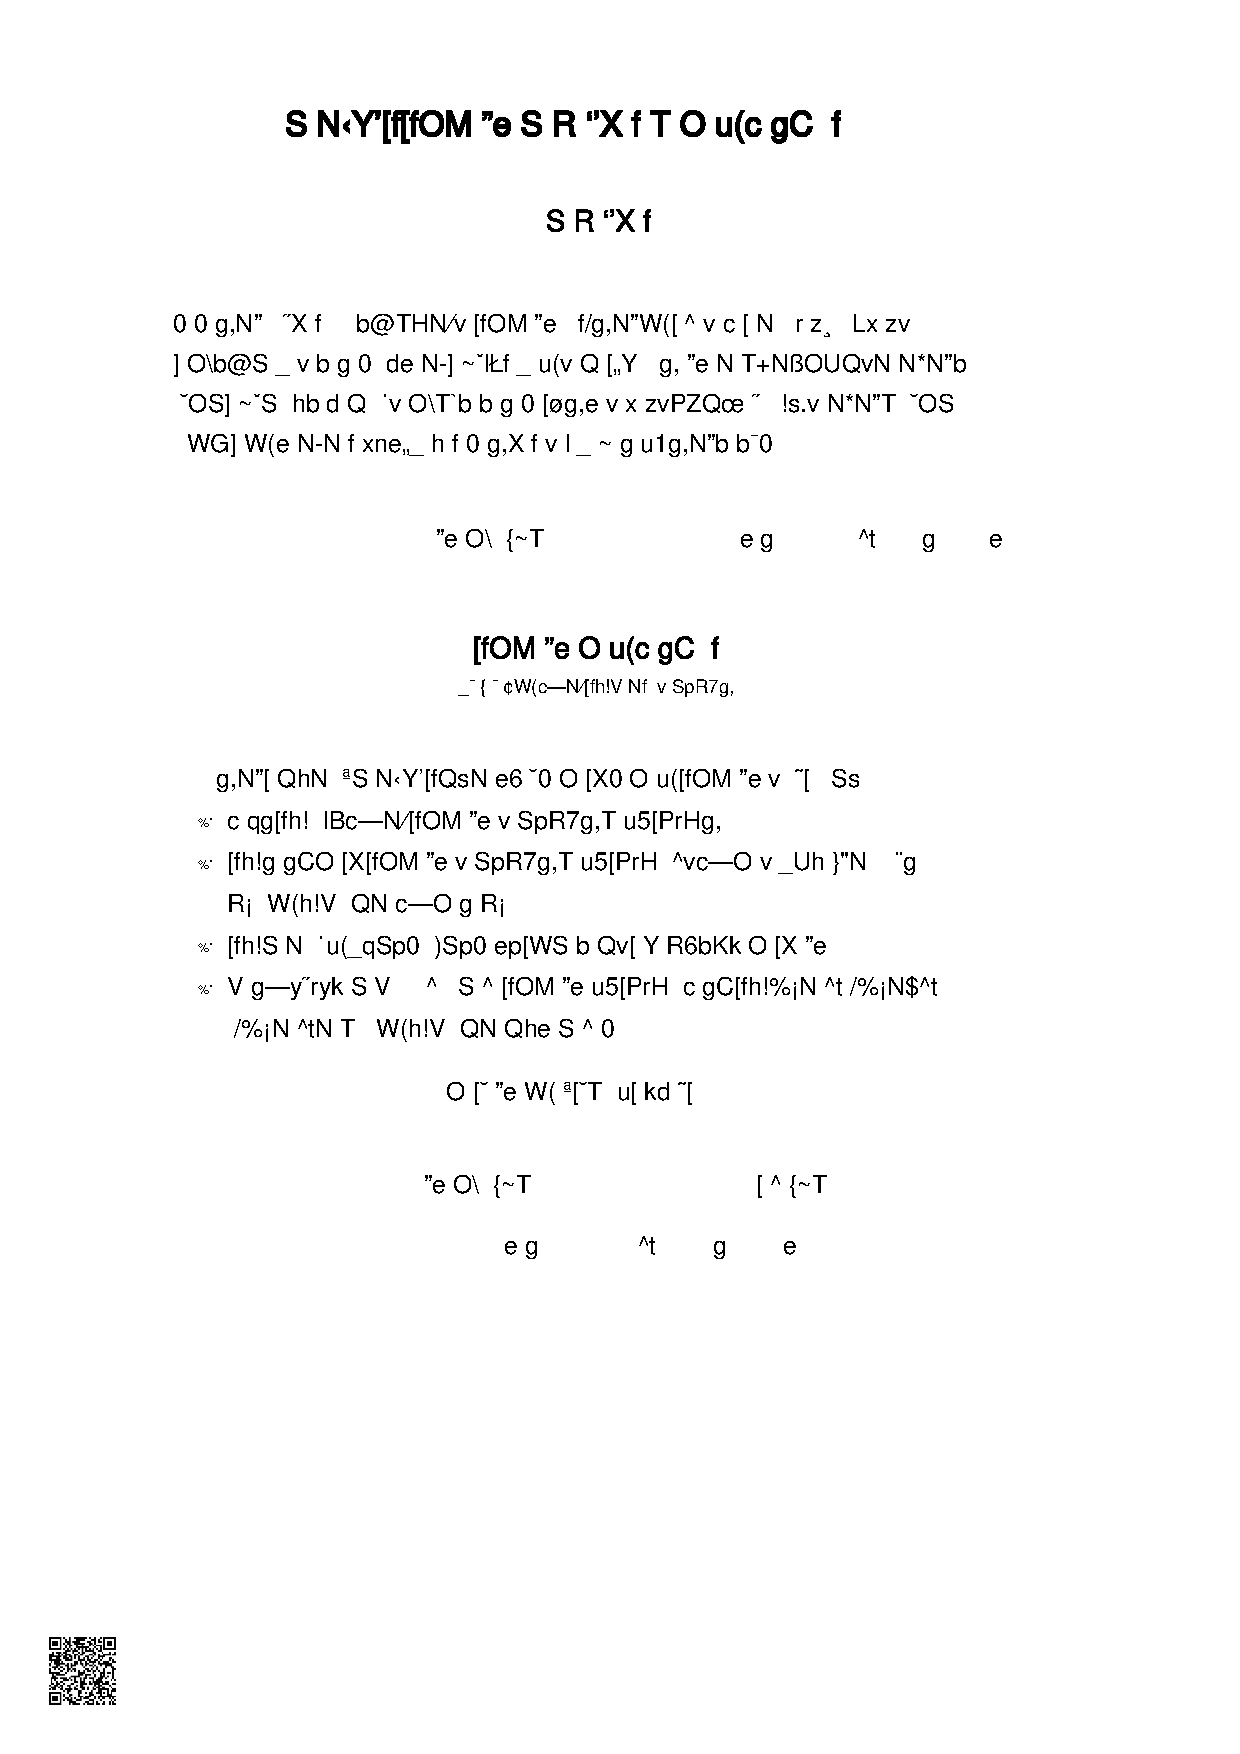
\includegraphics[height = 1.2448\textheight]{原创性声明.pdf}
		}
	\end{textblock}
}

% vim:ts=4:sw=4

\pkuthssinfo{
    cthesisname = {硕士学位论文},
    thesiscover = {硕士研究生学位论文},
    ethesisname = {Master Thesis},
    ctitle = {\zhtitle},
    etitle = {\entitle},
    cauthor = {\zhauthor}, eauthor = {\enauthor},
    studentid = {\thestudentid},
    % 具体时间以教务为准,初稿3月,送审4月,答辩5月,最终6月。
    date = {\zhdigits{\theyear}\ \ 年\ \ \zhnumber{\themonth}\ \ 月}, % June, 2022
    school = {汇丰商学院},
    cmajor = {\zhmajor}, emajor = {\enmajor},
    direction = {\majordirection},
    % 副教授 A.P. 讲师 Lec.
    cmentor = {\zhmentor}, ementor = {\enmentor},
    ckeywords = {\zhkeywords}, ekeywords = {\enkeywords},
    % 盲审模式参数, 需在documentclass增加blind
    % blindid = {XXXXXXXXX}, discipline = {XXXX}
}


\addbibresource{ref.bib}


\begin{document}
    \frontmatter
    \pagestyle{empty}
    % \maketitle
    % \cleardoublepage
    % 需替换门户版权声明pdf
    % % Copyright (c) 2008-2009 solvethis
% Copyright (c) 2010-2017,2021 Casper Ti. Vector
% Copyright (c) 2021 iofu728
% All rights reserved.
%
% Redistribution and use in source and binary forms, with or without
% modification, are permitted provided that the following conditions are
% met:
%
% * Redistributions of source code must retain the above copyright notice,
%   this list of conditions and the following disclaimer.
% * Redistributions in binary form must reproduce the above copyright
%   notice, this list of conditions and the following disclaimer in the
%   documentation and/or other materials provided with the distribution.
% * Neither the name of Peking University nor the names of its contributors
%   may be used to endorse or promote products derived from this software
%   without specific prior written permission.
%
% THIS SOFTWARE IS PROVIDED BY THE COPYRIGHT HOLDERS AND CONTRIBUTORS "AS
% IS" AND ANY EXPRESS OR IMPLIED WARRANTIES, INCLUDING, BUT NOT LIMITED TO,
% THE IMPLIED WARRANTIES OF MERCHANTABILITY AND FITNESS FOR A PARTICULAR
% PURPOSE ARE DISCLAIMED. IN NO EVENT SHALL THE COPYRIGHT HOLDER OR
% CONTRIBUTORS BE LIABLE FOR ANY DIRECT, INDIRECT, INCIDENTAL, SPECIAL,
% EXEMPLARY, OR CONSEQUENTIAL DAMAGES (INCLUDING, BUT NOT LIMITED TO,
% PROCUREMENT OF SUBSTITUTE GOODS OR SERVICES; LOSS OF USE, DATA, OR
% PROFITS; OR BUSINESS INTERRUPTION) HOWEVER CAUSED AND ON ANY THEORY OF
% LIABILITY, WHETHER IN CONTRACT, STRICT LIABILITY, OR TORT (INCLUDING
% NEGLIGENCE OR OTHERWISE) ARISING IN ANY WAY OUT OF THE USE OF THIS
% SOFTWARE, EVEN IF ADVISED OF THE POSSIBILITY OF SUCH DAMAGE.

% 此处不用 \specialchap,因为学校要求目录不包括其自己及其之前的内容。
\chapter*{版权声明}
% 综合学校的书面要求及 Word 模版来看,版权声明页不用加页眉、页脚。
\thispagestyle{empty}

任何收存和保管本论文各种版本的单位和个人,
未经本论文作者同意,不得将本论文转借他人,
亦不得随意复制、抄录、拍照或以任何方式传播。
否则一旦引起有碍作者著作权之问题,将可能承担法律责任。

% 替换门户下载pdf
\begin{textblock}{1}(-0.8,-0.08)
    \colorbox{white}{
        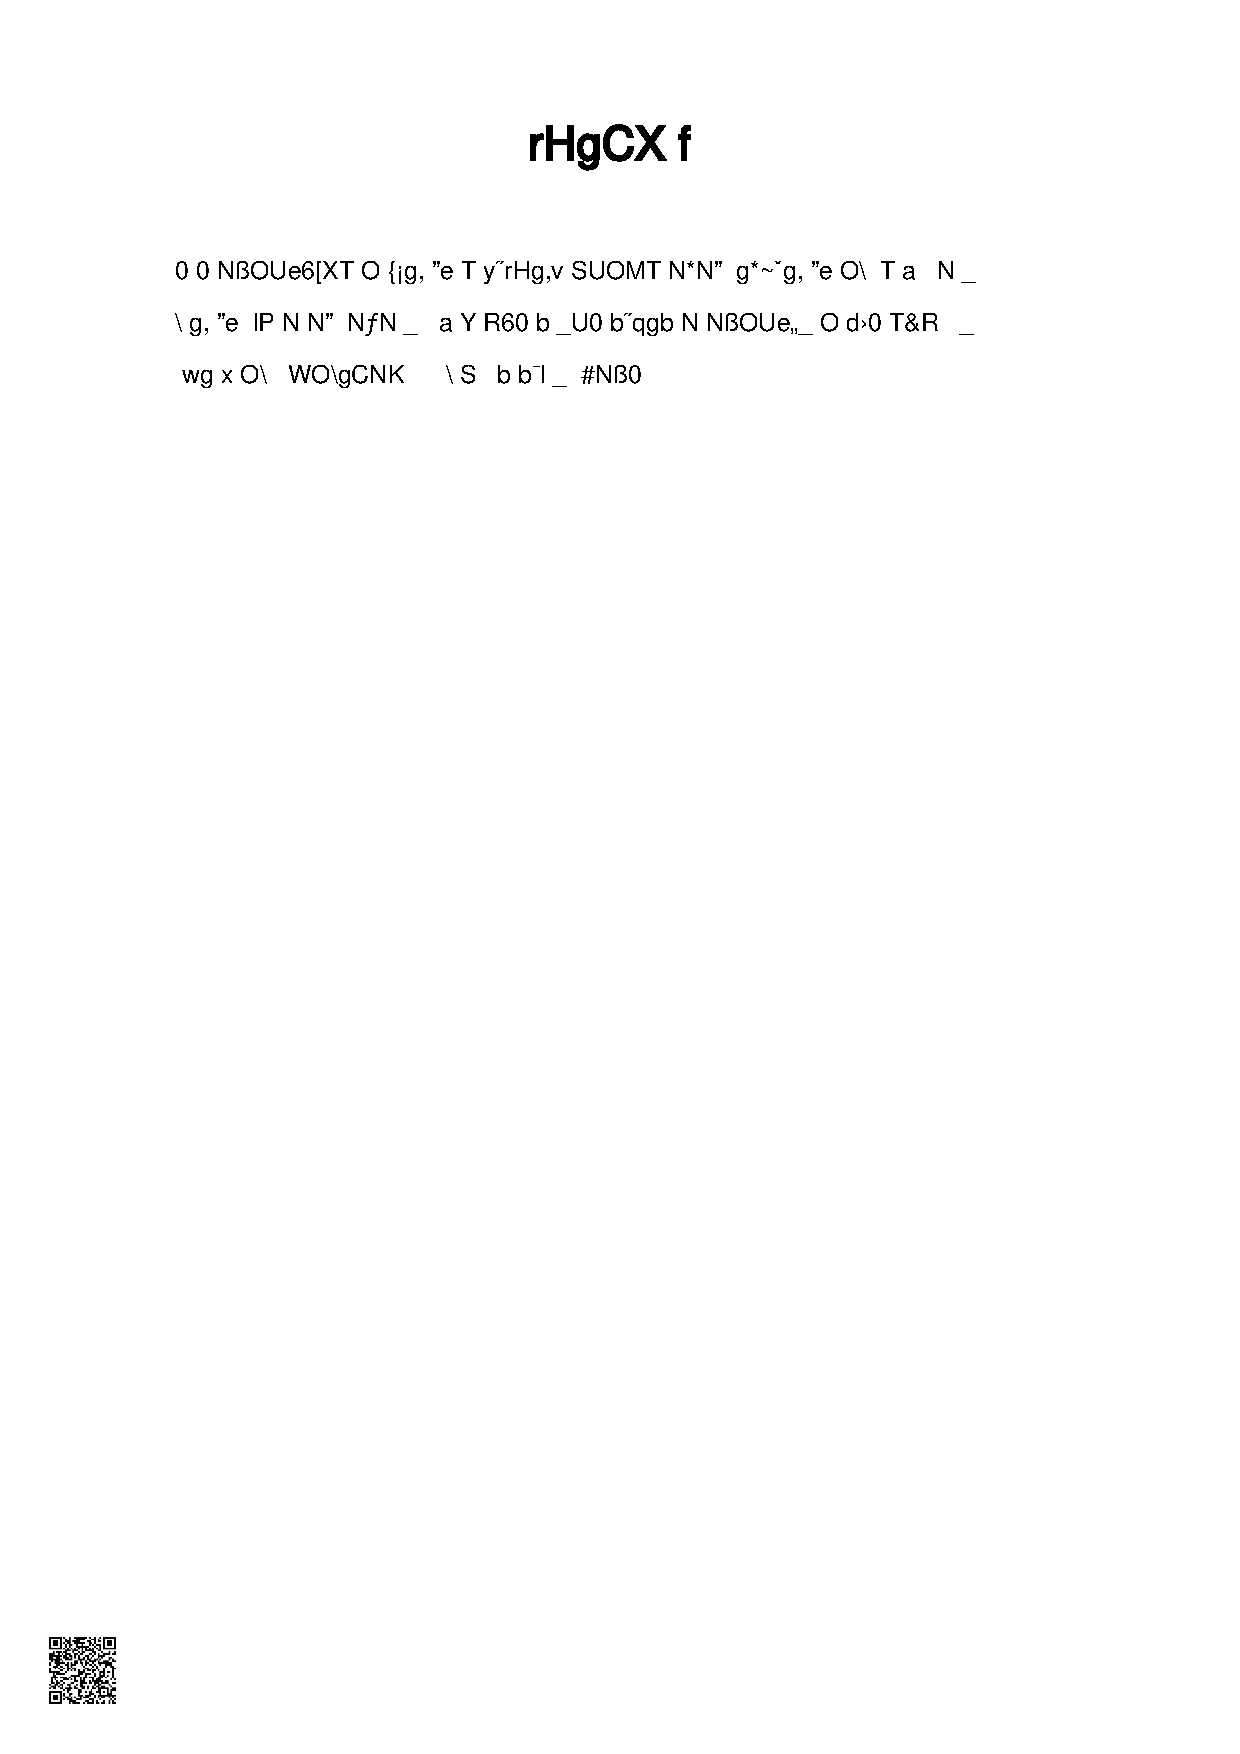
\includegraphics[height = 1.2448\textheight]{版权声明.pdf}
    }
\end{textblock}

% vim:ts=4:sw=4

    \cleardoublepage
    \pagestyle{plain}
    \setcounter{page}{0}
    \pagenumbering{Roman}
    \begin{cabstract}
	\addcontentsline{toc}{chapter}{摘要}

	在现代工作环境中,“摸鱼”现象,即员工在工作时间从事非工作相关事务或降低工作投入度的行为,日益普遍。这种现象不仅影响组织效率,也反映了雇佣关系中深刻的经济学问题。本文从{信息经济学}的视角出发,基于{委托代理理论}和{博弈论},探讨在{信息不对称}环境下,员工如何选择最优的“{摸鱼}”策略,以及雇主如何设计最优的{激励}与{监督}机制。研究旨在揭示该行为的内在经济逻辑,并为理解和管理现代劳动关系提供理论依据与(模拟的)实证参考。

	本文首先构建了一个简约的理论模型。在该模型中,风险中性的雇主无法直接观测风险中性雇员的努力程度,但可以通过设定最低努力标准、支付固定工资,并辅以概率性{监督}和惩罚机制来激励雇员。模型推导表明,雇员的最优决策呈现门槛效应:只有当预期惩罚(监督概率乘以惩罚力度)超过达到最低努力标准的成本时,雇员才会选择恰好达到该标准;否则,将选择完全不努力(最大化“摸鱼”)。进而,模型分析了雇主在权衡产出收益、工资支付和监督成本后,如何选择最优的最低努力要求和监督概率。

	为检验理论模型的启示,本文利用(虚构的)“中国企业员工调查(CEES)”面板数据,构建了固定效应计量模型进行实证分析。结果显示:企业{监督}强度的提高和{绩效工资}占比的增加,均与员工“摸鱼”指数呈显著负相关,验证了{监督}和{激励}对约束机会主义行为的有效性;而任务复杂度的提高则与“摸鱼”指数呈正相关,可能反映了复杂工作更难被有效监督的特性。

	研究结合了理论推导与(虚构的)实证检验,深化了对{信息不对称}下“摸鱼”行为经济根源的理解。研究结果为企业管理者设计更有效的{激励}机制(如平衡绩效薪酬与监督投入)和管理策略(如针对不同复杂度工作采取差异化管理方式)提供了启示。本文强调,理解“摸鱼”的经济学原理,并非鼓励该行为,而是旨在通过科学分析促进更和谐、高效的劳资关系。
\end{cabstract}

% vim:ts=4:sw=4

    \addcontentsline{toc}{chapter}{目录}
    \tableofcontents

    \mainmatter
    \chapter{引论}

\section{研究背景}

在现代组织管理实践中,员工的\zhquote{摸鱼}(或称\zhquote{在岗磨洋工}、\zhquote{工作规避})现象日益引起关注。它指的是员工在工作时间内,并未完全投入到与工作职责直接相关的任务中,而是从事非工作活动、降低努力程度或拖延工作进度的行为。这种现象并非简单的个人惰性问题,而是根植于复杂的组织环境和雇佣关系之中,尤其是在雇主(委托人)与雇员(代理人)之间普遍存在{信息不对称}的情况下 \citep{akerlof1970market, spence1973job}。雇主往往难以精确观测和衡量员工的实际努力水平和时间投入,这为员工提供了选择性投入努力、寻求个人效用最大化(例如,追求闲暇、处理私人事务)的空间,即采取某种程度的\zhquote{摸鱼}行为 \citep{alchian1972production}。

虽然\zhquote{摸鱼}现象普遍存在,但其背后的经济学原理,特别是员工如何在信息不对称的环境下做出\zhquote{最优}的摸鱼决策,以及这种决策如何与企业的激励机制和监督策略相互作用,尚未得到充分和系统的探讨。现有的管理学和组织行为学文献多从心理、文化或管理技巧角度分析 \citep[例如][]{ashforth1990social, robbins2016organizational},而经济学文献虽有大量关于委托代理模型和激励理论的研究 \citep{holmstrom1979moral, grossman1983analysis},但将这些理论精细化应用于分析日常工作场景中普遍存在的、程度可变的\zhquote{摸鱼}行为,并明确探讨其\zhquote{最优性}问题,以及雇主的最优应对策略,仍有较大的研究空间。特别是,结合理论模型与实证检验来理解这一现象的研究相对不足。理解这一行为的内在经济逻辑,对于设计更有效的管理制度、优化人力资源配置、提升组织整体效率具有重要的理论和现实意义。

本研究尝试从{信息经济学}和{博弈论}的视角切入,将\zhquote{摸鱼}视为员工在面临不完全信息和特定激励约束下的理性(或有限理性)决策过程。我们旨在构建一个理论框架,用以分析员工如何权衡努力付出的成本、被发现并惩罚的风险以及\zhquote{摸鱼}带来的效用,从而选择一个对其自身而言最优的努力水平。同时,本研究也将考察雇主如何设计包括{监督}强度和努力要求在内的契约来应对这种行为,以及双方策略互动最终可能达到的均衡状态。此外,本研究还将利用(虚构的)实证数据,检验理论模型提出的部分核心机制。

\section{研究问题}

基于上述背景和后续章节的分析框架,本研究旨在探讨以下核心问题:

\begin{enumerate}
    \item 在雇主无法完全观测雇员努力程度的信息不对称条件下,员工的\zhquote{最优摸鱼}策略(在此简化模型中体现为努力水平的选择)如何决定?哪些因素(如监督概率、惩罚力度、努力成本)是关键?
    \item 雇主如何设计最优的{监督}与{激励}契约(在此简化模型中体现为最低努力要求 $e_{min}$、监督概率 $p$ 和固定工资 $w$)来应对员工的潜在\zhquote{摸鱼}行为,以最大化自身利润?最优契约参数如何受到外部因素(如监督成本、惩罚上限、努力成本参数)的影响?
    \item (基于虚构数据的实证分析)在现实(模拟)环境中,企业的监督强度、绩效薪酬的激励力度以及工作任务本身的特征(如复杂度)与员工的\zhquote{摸鱼}行为之间存在怎样的关系?理论预测是否能在(虚构的)数据中得到支持?
\end{enumerate}

\section{研究贡献}

本研究预期在以下几个方面做出贡献:

首先,在{理论层面},将经典的{委托代理理论}和{博弈论}模型应用于分析\zhquote{摸鱼}这一具体而普遍的现代职场现象,深化对信息不对称下员工机会主义行为的理解。通过明确探讨\zhquote{最优摸鱼}策略(在此模型中是达到最低标准或完全不努力的二元选择)的形成机制及其对监督和惩罚的反应,为劳动经济学和组织经济学提供分析视角。

其次,在{模型构建与分析层面},本研究构建了一个简约但清晰的理论模型,内生化了雇员的努力选择和雇主的部分契约设计(最低努力标准和监督概率),并进行了详细的均衡分析和比较静态分析,揭示了关键参数对均衡结果的影响机制。

再次,在{结合理论与(虚构)实证层面},本研究不仅构建理论模型,还通过(虚构的)面板数据和固定效应计量模型,对理论提出的一些核心关系(如监督、绩效激励对摸鱼的抑制作用,以及任务复杂度的潜在影响)进行了实证检验,展示了理论指导实证、实证反馈理论的研究思路。

最后,在{实践启示层面},研究结论(包括理论和虚构实证部分)为企业管理者提供了关于员工行为的洞见。理解\zhquote{摸鱼}的经济根源和影响因素,有助于管理者设计更有效的监督策略、激励机制(如平衡监督成本与激励效果、考虑工作特性),从而在控制机会主义行为与维持组织效率之间找到更合适的平衡点。

\section{论文结构安排}

本文的后续结构安排如下:第二章将回顾相关文献,梳理委托代理理论、博弈论、激励理论以及组织行为学中关于员工努力、监督和机会主义行为的研究,为本研究定位。第三章将详细介绍本文构建的理论模型,包括基本假设(如风险中性、特定成本函数)、变量定义、模型设定。第四章将对模型进行深入分析,推导雇员的最优努力决策规则、雇主的最优契约设计(最低努力标准、监督概率和工资),并进行比较静态分析。第五章将展示基于(虚构的)中国企业员工调查数据的实证研究,包括模型设定、变量说明、基准回归结果及稳健性讨论,检验理论模型的部分预测。第六章总结全文研究结论,讨论其理论意义与实践启示,并指出研究的局限性(如模型简化、数据虚构等)与未来可能的研究方向。
    \chapter{Literature Review}

This chapter aims to systematically review the theoretical and empirical research related to employee \enquote{shirking} behavior, laying the groundwork for subsequent model construction and analysis. We will primarily focus on reviewing literature concerning principal-agent theory, incentive and contract theory, the application of game theory in employment relationships, and relevant studies in organizational behavior regarding employee motivation and opportunism.

\section{Principal-Agent Theory and Information Asymmetry}

One of the core features of modern corporate organizations is the separation of ownership and control, which forms the basis of the principal-agent relationship \citep{jensen1976theory}. In this relationship, the principal (e.g., employer, shareholder) delegates decision-making authority or task execution power to the agent (e.g., employee, manager), expecting the agent to act in the best interest of the principal. However, due to information asymmetry, particularly the difficulty for the principal to fully observe and verify the agent's actions (such as effort level), the agent may leverage this informational advantage to pursue their own interests, leading to the problem of Moral Hazard \citep{holmstrom1979moral}.

Employee \enquote{shirking} behavior can be considered a typical manifestation of moral hazard. Because employers cannot precisely monitor every activity and effort input of their employees, employees may choose to exert less effort than agreed upon or expected, use work time for non-work matters, or complete tasks with lower efficiency, i.e., \enquote{Shirking} on the job \citep{alchian1972production}. Akerlof's \enquote{market for lemons} theory \citep{akerlof1970market} and Spence's signaling theory \citep{spence1973job} also reveal how information asymmetry affects market efficiency and individual behavior, principles that equally apply within the labor market. To mitigate problems arising from information asymmetry, principals need to design mechanisms to monitor agent behavior or incentivize effort exertion.

Early principal-agent models typically assumed that the agent's effort is unobservable, and the principal can only observe an output signal related to effort, which is also subject to random disturbances \citep{holmstrom1979moral, grossman1983analysis}. This made incentive contracts based on output the focus of research. Studies show that optimal contract design requires a trade-off between risk sharing and providing incentives. When agents are risk-averse, transferring excessive risk to them reduces their utility and requires a higher risk premium; insufficient incentives, however, lead agents to choose suboptimal effort levels.

\section{Incentive Theory and Contract Design}

To address the agency problem, economists have developed a rich body of incentive theory. The core idea is to align the agent's interests with the principal's objectives through the design of effective contracts.

Performance Pay is one of the most widely applied incentive tools. Theoretical research and empirical evidence suggest that linking compensation to measurable performance indicators can significantly increase employee effort and productivity \citep{lazear1999performance}. However, designing performance pay faces numerous challenges, such as: the measurability issue of performance indicators (output of some tasks is difficult to quantify), the multi-task problem (employees may focus only on tasks with easily measured performance while neglecting other important responsibilities), and potential inducements for short-term behavior and excessive competition \citep{holmstrom1991multitask}.

Efficiency Wage Theory offers another perspective. It posits that employers paying wages above the market-clearing level can increase the opportunity cost of shirking for employees (i.e., the cost of losing a high-paying job), thereby motivating them to work harder and reducing the need for supervision \citep{shapiro1984equilibrium}. Efficiency wages can also attract higher-quality employees, reduce turnover rates, and enhance employee morale and sense of fairness \citep{akerlof1986efficiency}.

Furthermore, non-monetary incentives such as promotions, career development, and reputation mechanisms also play important roles in the employment relationship \citep{fama1980agency, gibbons1999careers}. Long-term employment relationships, internal labor markets, and corporate culture, by fostering trust and repeated interactions, can mitigate short-term opportunistic behavior to some extent.

The development of contract theory has also gradually moved from assumptions of perfect rationality and complete contracts towards acknowledging the reality of bounded rationality and contract incompleteness \citep{hart1995firms}. The concept of the Psychological Contract emphasizes the implicit expectations and mutual obligations in the employment relationship that are not explicitly written into formal contracts \citep{rousseau1995psychological}. When employees perceive that the organization has violated the psychological contract (e.g., broken promises, unfair treatment), their work motivation, loyalty, and effort levels may significantly decrease, making them more prone to negative behaviors such as \enquote{shirking}.

\section{Game Theory Perspective on the Employment Relationship}

The employment relationship can be viewed as an ongoing game between the employer and the employee. Both parties, operating under conditions of incomplete information, choose their optimal actions based on expectations of the other party's strategies.

Incorporating \enquote{shirking} behavior into a game-theoretic framework helps analyze the interaction of strategies and equilibrium outcomes. For instance, the employer's monitoring strategy (e.g., frequency, intensity) and the employee's shirking strategy (e.g., degree, method) can be treated as interdependent decision variables. Increased monitoring investment by the employer can raise the probability of detecting shirking, thus deterring such behavior, but monitoring itself is costly. The employee, in turn, must weigh the utility gained from shirking against the risk of detection and the cost of working diligently. Tirole's (1986) \nocite{tirole1986hierarchies} research on collusion within organizations also suggests that monitoring systems themselves may have loopholes, potentially allowing for some form of \enquote{collusion} between managers and employees that affects monitoring effectiveness.

Repeated game models are particularly suitable for analyzing long-term employment relationships. In repeated games, reputation mechanisms and retaliatory strategies (such as \enquote{trigger strategies}) can support cooperative equilibria, where employees choose not to shirk, and employers choose to trust or monitor less \citep{axelrod1984evolution}. However, maintaining cooperative equilibrium requires certain conditions, such as a sufficiently long game duration (or low probability of termination), sufficient patience from both parties (discount factor not too low), and adequate information transparency.

\section{Organizational Behavior and Psychological Perspectives}

Economic models typically assume individuals are rational and self-interested, seeking to maximize utility. In contrast, organizational behavior and psychology offer richer explanations for employee motivation and behavior.

Besides external incentives (like wages, bonuses), Intrinsic Motivation—the enjoyment, sense of achievement, autonomy, etc., derived from the work itself—is also a significant driver of employee effort \citep{deci1985intrinsic}. Over-reliance on external controls and monitoring can sometimes undermine employees' intrinsic motivation, leading to the so-called \enquote{crowding-out effect} of incentives \citep{frey1997not}.

Factors such as Burnout, Organizational Justice, Leadership Style, and Organizational Culture have also been shown to be closely related to employee work attitudes and behaviors (including work engagement, absenteeism, turnover intention, and counterproductive work behaviors like \enquote{shirking}) \citep{maslach2001job, colquitt2001organizational}. For example, when employees perceive distributive or procedural injustice, they might \enquote{correct} this perceived unfairness by reducing effort or increasing non-work activities. \enquote{Cyberloafing}, the use of company-provided internet access for non-work-related online activities during work hours, has emerged as a new research hotspot in modern workplaces \citep{lim2002it}.

\section{Literature Summary and Research Positioning}

In summary, the existing literature has explored the theoretical foundations and influencing factors related to employee \enquote{shirking} behavior from various disciplinary perspectives. Principal-agent theory reveals the roots of information asymmetry and moral hazard; incentive theory examines how to guide employee behavior through contract design; game theory analyzes the strategic interactions between employers and employees; and organizational behavior emphasizes the role of psychological factors and the organizational environment.

However, current research still exhibits some limitations:
1.  Most economic models tend to treat effort/shirking as a discrete choice (e.g., effort/no effort) or focus on specific types of shirking (e.g., reducing output quantity/quality), with fewer models formalizing the decision-making process where employees choose the *degree* of \enquote{shirking} continuously or multi-dimensionally.
2.  Research that endogenizes both the employee's individual \enquote{optimal shirking} decision and the employer's optimal incentive/monitoring strategy within the same theoretical framework, analyzing their interactive equilibrium, is relatively scarce.
3.  There is a lack of fine-grained theoretical characterization regarding how the \enquote{degree} of \enquote{shirking} is determined, i.e., how employees seek an optimal balance between pursuing personal leisure utility and maintaining job security/avoiding punishment.

Building upon previous research, this study attempts to focus on the issue of employee \enquote{optimal shirking} strategy choice in an environment of asymmetric information. We will construct a theoretical model that explicitly treats the degree of \enquote{shirking} as a continuous decision variable for the employee, analyzing how it is influenced by factors such as wage structure, monitoring probability, punishment severity, job characteristics, and individual preferences. Concurrently, the model will also incorporate the employer's incentive and monitoring strategies as endogenous variables to examine the equilibrium outcome under the strategic interaction of both parties. The aim is to provide a more refined economic analysis framework for understanding the ubiquitous phenomenon of \enquote{shirking} in the modern workplace and to offer theoretical insights for designing more effective management strategies.
    \chapter{理论模型构建}
\label{chap:model}

本章旨在构建一个理论模型,刻画信息不对称下雇员的\zhquote{摸鱼}(即选择努力程度)行为以及雇主的最优应对策略。模型将借鉴委托代理理论和博弈论的基本框架。

\section{模型基本设定}
\label{sec:model_setup}

考虑一个单一周期(single-period)的雇佣关系,参与者包括一个风险中性(risk-neutral)的雇主(委托人,Principal, P)和一个同样是风险中性的雇员(代理人,Agent, A)。雇员拥有保留效用(reservation utility) $\bar{U}$,代表其接受雇佣关系的最低效用水平,为简化分析,我们将其标准化为 $\bar{U} = 0$。

博弈顺序如下:
\begin{enumerate}
    \item  雇主设计并提供一份雇佣契约给雇员。
    \item  雇员决定是否接受契约。如果拒绝,雇员获得保留效用 $\bar{U}=0$,雇主获得0利润。如果接受,博弈继续。
    \item  雇员选择其努力程度 $e$。努力程度 $e \ge 0$。同时,雇员付出努力会产生相应的成本。
    \item  产出 $q$ 实现,支付根据契约执行。
\end{enumerate}

核心假设是信息不对称:雇主无法直接观测到雇员选择的努力程度 $e$。但是,雇主可以通过监督机制(monitoring)或观察最终产出 $q$ 来间接推断或影响雇员的努力选择。

\subsection{雇员的努力与成本}

雇员选择努力程度 $e$。我们假设努力程度是一个连续变量,$e \in [0, \infty)$。付出努力会给雇员带来负效用(成本)。我们用成本函数 $c(e)$ 来表示,并假设该函数具有以下性质:
\begin{itemize}
    \item $c(0) = 0$:不付出努力则没有成本。
    \item $c'(e) > 0$ for $e > 0$:努力成本随努力程度的增加而增加(边际成本为正)。
    \item $c''(e) > 0$:努力的边际成本递增(成本函数是严格凸函数)。
\end{itemize}
A commonly used form for the cost function is $c(e) = \frac{k}{2}e^2$, where $k > 0$ 是一个成本参数,反映了努力的困难程度。

雇员的\zhquote{摸鱼}程度可以视为其选择的努力水平 $e$ 相对于某个基准(例如,雇主期望的水平或最大可能水平)的偏离。在本模型中,我们直接分析雇员的最优努力 $e$ 的选择。

\subsection{产出与支付}

为简化模型,我们首先考虑一个确定性产出(deterministic output)的情形,即产出 $q$ 完全由雇员的努力程度决定:
\begin{equation}
q = e
\end{equation}
这意味着雇主可以通过观察产出 $q$ 来完美推断努力 $e$。在这种情况下,不存在信息不对称,雇主可以通过设计一个强制特定努力水平 $e^*$ 并支付相应工资的契约来达到最优。例如,规定如果 $q=e^*$ 则支付 $w$,否则支付0或进行惩罚。只要 $w - c(e^*) \ge 0$,雇员就会接受并选择 $e=e^*$。

然而,现实中产出往往受到随机因素的影响。一个更现实的设定是随机产出(stochastic output),例如:
\begin{equation}
q = e + \epsilon
\end{equation}
其中 $\epsilon$ 是一个均值为0的随机噪声项(例如,服从正态分布 $N(0, \sigma^2)$)。在这种情况下,即使观察到产出 $q$,雇主也无法完全确定雇员的努力 $e$,信息不对称问题凸显。

契约可以基于可观测的变量,如产出 $q$ 或通过监督获得的信息。常见的契约形式包括:
\begin{itemize}
    \item 固定工资契约(Fixed Wage Contract):无论产出如何,支付固定工资 $w$。
    \item 线性绩效工资契约(Linear Performance Pay Contract):工资 $w = s + bq$,其中 $s$ 是固定部分,$b$ 是基于产出的佣金率(bonus rate)。
    \item 基于监督的契约(Monitoring-Based Contract):雇主以一定概率 $p$ 进行监督。如果监督发现雇员行为不符合要求(例如,努力低于某个标准 $e^*$),则进行惩罚。
\end{itemize}

\section{雇员行为分析:固定工资与监督}
\label{sec:agent_behavior_monitor}

现在我们分析在一个相对简单的契约结构下,雇员如何选择其最优努力程度。考虑雇主提供一份包含固定工资 $w$ 和监督惩罚机制的契约。

具体地,雇主以概率 $p \in [0, 1]$ 对雇员进行监督。监督是完美的,一旦实施,就能准确观测到雇员的实际努力程度 $e$。契约规定了一个最低努力标准 $e_{min} \ge 0$。如果雇员被监督到,且其努力程度 $e < e_{min}$,则雇员需要承担一个惩罚 $F > 0$(例如,罚款、扣减工资等)。如果 $e \ge e_{min}$,或者雇员没有被监督到(概率为 $1-p$),则不会受到惩罚。

假设雇员是风险中性的,其目标是最大化其期望效用。雇员的效用来自于获得的工资,减去努力成本,再减去可能的期望惩罚。给定契约 $(w, p, e_{min}, F)$,雇员选择努力 $e$ 来最大化:
\begin{equation}
E[U(e)] = w - c(e) - p \cdot \mathbb{I}(e < e_{min}) \cdot F
\end{equation}
其中 $\mathbb{I}(\cdot)$ 是指示函数,当条件成立时取值为1,否则为0。

雇员的最优决策如下:
\begin{enumerate}
    \item  如果选择 $e \ge e_{min}$**:此时 $\mathbb{I}(e < e_{min}) = 0$,雇员不会受到惩罚。其效用为 $U_1(e) = w - c(e)$。为了最大化效用,雇员会选择满足 $e \ge e_{min}$ 约束下的最低成本努力,即选择 $e = e_{min}$。此时的效用为 $U_1^* = w - c(e_{min})$。

    \item  如果选择 $e < e_{min}$**:此时 $\mathbb{I}(e < e_{min}) = 1$,雇员面临被发现并惩罚的风险。其期望效用为 $E[U_2(e)] = w - c(e) - pF$。为了最大化这个期望效用,雇员会选择成本最低的努力,即 $e=0$(假设 $e=0$ 是允许的最低努力)。此时的期望效用为 $E[U_2^*] = w - c(0) - pF = w - pF$。
\end{enumerate}

雇员将在上述两种情况中选择能带来更高(期望)效用的那个:
雇员会选择 $e = e_{min}$ 当且仅当
\begin{equation}
U_1^* \ge E[U_2^*]
\end{equation}
\begin{equation}
w - c(e_{min}) \ge w - pF
\end{equation}
\begin{equation}
pF \ge c(e_{min})
\end{equation}

{结论}:在该契约下,雇员的最优努力选择 $e^*$ 是:
\begin{equation}
e^* = \begin{cases} e_{min} & \text{if } pF \ge c(e_{min}) \\ 0 & \text{if } pF < c(e_{min}) \end{cases}
\end{equation}

这个结果直观地说明了:只有当预期的惩罚(被发现的概率 $p$ 乘以惩罚力度 $F$)足够大,能够超过达到最低努力标准 $e_{min}$ 所需的成本 $c(e_{min})$ 时,雇员才会被激励去达到这个标准。否则,雇员宁愿选择完全不努力($e=0$),并承担 $pF$ 的预期惩罚成本,因为这样做可以节省 $c(e_{min})$ 的努力成本。

这个简单的模型揭示了监督和惩罚在约束\zhquote{摸鱼}行为中的作用,但也显示了其局限性:它只能激励雇员达到最低标准 $e_{min}$,而无法激励更高的努力水平。并且,努力的选择呈现一个\zhquote{全有或全无}(相对于 $e_{min}$ 而言)的特征。

% 下一节将分析雇主如何设计最优契约
    \chapter{模型分析}
\label{chap:analysis}

基于第三章构建的理论模型,本章将深入分析雇员的最优努力决策及其影响因素,并探讨雇主在信息不对称背景下如何设计最优的契约(特别是监督强度和最低努力标准)来最大化自身利润。

\section{雇员最优努力决策分析}
\label{sec:agent_decision_analysis}

回顾第三章 \ref{sec:agent_behavior_monitor} 的分析结果,在固定工资 $w$、监督概率 $p$、最低努力标准 $e_{min}$ 和惩罚 $F$ 的契约下,风险中性的雇员会比较选择 $e=e_{min}$ 的效用 $U_1^* = w - c(e_{min})$ 与选择 $e=0$ 的期望效用 $E[U_2^*] = w - pF$。

最终的决策规则是(如公式 \ref{eq:agent_choice_recap} 所示):
\begin{equation} \label{eq:agent_choice_recap}
e^* = \begin{cases} e_{min} & \text{if } pF \ge c(e_{min}) \\ 0 & \text{if } pF < c(e_{min}) \end{cases}
\end{equation}

这个结果揭示了几个关键点:
\begin{enumerate}
    \item \textbf{监督与惩罚的门槛效应}:雇员是否选择达到最低努力标准 $e_{min}$,完全取决于预期的惩罚 $pF$ 是否足以覆盖达到该标准所需的努力成本 $c(e_{min})$。这是一个明显的门槛效应(threshold effect)。只有当监督概率 $p$ 和惩罚力度 $F$ 的乘积跨过 $c(e_{min})$ 这个门槛时,雇员的行为才会从完全不努力($e=0$,最大化\zhquote{摸鱼})跳跃到恰好满足最低要求的努力($e=e_{min}$)。
    \item \textbf{无法激励超额努力}:该机制只能激励雇员达到最低标准 $e_{min}$,而无法激励其付出超过 $e_{min}$ 的努力。因为一旦达到 $e_{min}$,进一步增加努力只会增加成本 $c(e)$,而不会带来额外的收益或减少惩罚风险。这体现了单纯依赖\zhquote{底线监督}型契约在激励方面的局限性。
    \item \textbf{\zhquote{最优摸鱼}策略的二元性}:在此简单模型中,雇员的\zhquote{摸鱼}策略呈现出一种相对极端的二元选择:要么完全不努力($e=0$),要么恰好达到最低标准($e=e_{min}$)。不存在一个介于两者之间的\zhquote{部分摸鱼}的均衡状态。这主要是由于模型假设监督能完美识别是否低于 $e_{min}$,且惩罚是固定的。
\end{enumerate}

这一分析突显了 $p$, $F$, $e_{min}$ 以及成本函数 $c(\cdot)$ 在决定雇员努力行为中的核心作用。接下来,我们将从雇主的角度出发,分析其如何选择这些契约参数。

\section{雇主的契约设计问题}
\label{sec:principal_problem}

现在我们考虑雇主(P)的决策问题。雇主的目标是最大化其期望利润 $E[\pi]$。假设雇主是风险中性的。其利润等于产出减去支付给雇员的工资,再减去实施监督的成本。

我们采用第三章 (\ref{sec:model_setup}) 提出的确定性产出假设 $q=e$ 来简化分析雇主问题的第一步。后续可以扩展到随机产出情形。
假设监督成本与监督概率 $p$ 相关,我们设监督成本为 $M(p)$。为简化分析,假设 $M(p) = \gamma p$,其中 $\gamma > 0$ 是单位监督概率的成本系数。

雇主需要选择契约参数 $(w, p, e_{min}, F)$。然而,惩罚力度 $F$ 往往受到法律法规、员工赔付能力或企业声誉等外部因素的限制。因此,我们假设存在一个最大的可行惩罚 $F_{max}$,即 $0 \le F \le F_{max}$。为了最大化惩罚的威慑效果,理性的雇主通常会选择尽可能大的惩罚,即设定 $F = F_{max}$。因此,雇主的决策变量简化为 $(w, p, e_{min})$。

雇主的优化问题是:
\begin{equation}
\max_{w, p, e_{min}} \quad E[\pi] = e^* - w - \gamma p
\end{equation}
subject to:
\begin{enumerate}
    \item 激励相容约束 (Incentive Compatibility, IC): 雇员会根据公式 \ref{eq:agent_choice_recap} 选择最优努力 $e^*$。
    \begin{equation} \label{eq:ic_constraint}
    e^* = \begin{cases} e_{min} & \text{if } p F_{max} \ge c(e_{min}) \\ 0 & \text{if } p F_{max} < c(e_{min}) \end{cases}
    \end{equation}
    \item 参与约束 (Participation Constraint, PC): 雇员接受契约获得的期望效用必须不低于其保留效用 $\bar{U}=0$。
    \begin{equation} \label{eq:pc_constraint}
    E[U(e^*)] = w - c(e^*) - p \cdot \mathbb{I}(e^* < e_{min}) \cdot F_{max} \ge 0
    \end{equation}
\end{enumerate}
其中 $0 \le p \le 1$ 且 $e_{min} \ge 0$。

\section{最优契约分析:固定工资与监督}
\label{sec:optimal_contract_monitor}

雇主在决策时,实质上面临两种选择:要么设计一个契约来激励雇员选择 $e^*=e_{min}$(诱导努力策略),要么接受雇员选择 $e^*=0$(放任摸鱼策略)。

\textbf{策略一:诱导努力 $e^* = e_{min}$}

要使雇员选择 $e^* = e_{min}$,必须满足 IC 条件 $p F_{max} \ge c(e_{min})$。为了最小化监督成本 $\gamma p$,雇主会选择满足该条件的最低监督概率 $p$。即:
\begin{equation} \label{eq:optimal_p}
p^* = \frac{c(e_{min})}{F_{max}}
\end{equation}
这里隐含了假设 $c(e_{min}) \le F_{max}$,否则即使 $p=1$ 也无法满足条件。如果 $c(e_{min}) > F_{max}$,则无法通过此机制诱导 $e_{min}$ 的努力。我们假设 $F_{max}$ 足够大,使得 $p^* \le 1$ 可行。

在该情况下,雇员的努力为 $e^*=e_{min}$,其期望效用为 $E[U(e_{min})] = w - c(e_{min}) - p^* \cdot \mathbb{I}(e_{min} < e_{min}) \cdot F_{max} = w - c(e_{min})$。
为了满足 PC 约束 $w - c(e_{min}) \ge 0$,同时最小化工资成本,雇主会设定最低的可行工资:
\begin{equation} \label{eq:optimal_w_emin}
w^* = c(e_{min})
\end{equation}

此时,雇主的利润为:
\begin{equation} \label{eq:profit_emin}
\pi_1(e_{min}) = e_{min} - w^* - \gamma p^* = e_{min} - c(e_{min}) - \gamma \frac{c(e_{min})}{F_{max}}
\end{equation}
雇主还需要选择最优的 $e_{min}$ 来最大化 $\pi_1(e_{min})$。假设努力成本函数为 $c(e) = \frac{k}{2}e^2$ ($k>0$),则
\begin{equation}
\pi_1(e_{min}) = e_{min} - \frac{k}{2}e_{min}^2 - \gamma \frac{k e_{min}^2}{2 F_{max}} = e_{min} - \frac{k}{2} \left( 1 + \frac{\gamma}{F_{max}} \right) e_{min}^2
\end{equation}
对 $e_{min}$ 求一阶导数并令其为0:
\begin{equation}
\frac{d\pi_1}{de_{min}} = 1 - k \left( 1 + \frac{\gamma}{F_{max}} \right) e_{min} = 0
\end{equation}
解得最优的最低努力要求 $e_{min}^*$:
\begin{equation} \label{eq:optimal_emin}
e_{min}^* = \frac{1}{k \left( 1 + \frac{\gamma}{F_{max}} \right)}
\end{equation}
二阶导数为 $-k(1 + \gamma/F_{max}) < 0$,确实是最大值点。
将 $e_{min}^*$ 代入,可得此时的最优监督概率 $p^{**} = \frac{c(e_{min}^*)}{F_{max}} = \frac{k (e_{min}^*)^2}{2 F_{max}}$ 和最优工资 $w^{**} = c(e_{min}^*) = \frac{k}{2}(e_{min}^*)^2$。

\textbf{策略二:放任摸鱼 $e^* = 0$}

如果雇主设计的契约参数使得 $p F_{max} < c(e_{min})$,或者干脆设定 $p=0$ 且 $e_{min}>0$ (或 $e_{min}=0$),则雇员会选择 $e^*=0$。
此时,雇员的努力为 $e^*=0$,其期望效用为 $E[U(0)] = w - c(0) - p \cdot \mathbb{I}(0 < e_{min}) \cdot F_{max} = w - p \cdot \mathbb{I}(e_{min}>0) \cdot F_{max}$。
为了满足 PC 约束 $w - p \cdot \mathbb{I}(e_{min}>0) \cdot F_{max} \ge 0$,雇主会设定最低工资 $w^* = p \cdot \mathbb{I}(e_{min}>0) \cdot F_{max}$。
雇主的利润为 $E[\pi_0] = e^* - w^* - \gamma p = 0 - p \cdot \mathbb{I}(e_{min}>0) \cdot F_{max} - \gamma p$。
显然,要最大化这个利润(即最小化损失),雇主最优的选择是令 $p=0$。此时,雇员选择 $e^*=0$,工资 $w^*=0$,利润 $\pi_0 = 0$。

\textbf{雇主的最终决策}

雇主会比较实施策略一(诱导努力 $e_{min}^*$)能获得的最大利润 $\pi_1(e_{min}^*)$ 和实施策略二(放任摸鱼 $e=0$)获得的利润 $\pi_0 = 0$。
只有当 $\pi_1(e_{min}^*) > 0$ 时,雇主才会选择诱导努力的策略。即:
\begin{equation}
\pi_1(e_{min}^*) = e_{min}^* - \frac{k}{2} \left( 1 + \frac{\gamma}{F_{max}} \right) (e_{min}^*)^2 > 0
\end{equation}
将 $e_{min}^* = \frac{1}{k(1 + \gamma/F_{max})}$ 代入:
\begin{equation}
\frac{1}{k(1 + \gamma/F_{max})} - \frac{k}{2} \left( 1 + \frac{\gamma}{F_{max}} \right) \left[ \frac{1}{k(1 + \gamma/F_{max})} \right]^2 > 0
\end{equation}
\begin{equation}
\frac{1}{k(1 + \gamma/F_{max})} - \frac{1}{2k(1 + \gamma/F_{max})} > 0
\end{equation}
\begin{equation}
\frac{1}{2k(1 + \gamma/F_{max})} > 0
\end{equation}
这个条件总是成立的,因为 $k>0, \gamma>0, F_{max}>0$。

因此,在本模型的假设下(确定性产出 $q=e$,努力成本 $c(e)=\frac{k}{2}e^2$,监督成本 $M(p)=\gamma p$,风险中性),只要可以实施监督和惩罚 ($F_{max}>0, \gamma < \infty$),雇主总是会选择诱导一个正的最低努力水平 $e_{min}^* = \frac{1}{k(1 + \gamma/F_{max})}$,并设定相应的监督概率 $p^{**}$ 和工资 $w^{**}$,这比完全放任摸鱼(利润为0)要更优。

\section{参数变化对最优契约的影响(比较静态分析)}
\label{sec:comparative_statics}

我们来分析关键参数如何影响雇主选择的最优最低努力标准 $e_{min}^*$ 以及相应的监督和工资水平:

\begin{itemize}
    \item \textbf{努力成本系数 $k$ 的影响}:
      $\frac{\partial e_{min}^*}{\partial k} = -\frac{1}{k^2 (1 + \gamma/F_{max})} < 0$.
      当努力变得更加困难($k$ 增大)时,雇主会降低所要求的最低努力标准 $e_{min}^*$。因为诱导相同努力水平的成本(包括支付给员工的补偿 $w^*=c(e_{min})$ 和维持监督所需的预期惩罚 $p^* F_{max} = c(e_{min})$,后者影响监督成本)增加了。

    \item \textbf{监督成本系数 $\gamma$ 的影响}:
      $\frac{\partial e_{min}^*}{\partial \gamma} = -\frac{1}{k (1 + \gamma/F_{max})^2} \cdot \frac{1}{F_{max}} < 0$.
      当监督变得更加昂贵($\gamma$ 增大)时,雇主也会选择降低最低努力标准 $e_{min}^*$。因为提高 $e_{min}$ 需要更高的 $p^*$(见公式 \ref{eq:optimal_p}),这会导致更高的监督成本 $\gamma p^*$。为了节省监督成本,雇主会降低目标努力水平。

    \item \textbf{最大惩罚 $F_{max}$ 的影响}:
      $\frac{\partial e_{min}^*}{\partial F_{max}} = -\frac{1}{k (1 + \gamma/F_{max})^2} \cdot (-\frac{\gamma}{F_{max}^2}) = \frac{\gamma}{k F_{max}^2 (1 + \gamma/F_{max})^2} > 0$.
      当最大允许的惩罚力度增大($F_{max}$ 增大)时,雇主会设定更高的最低努力标准 $e_{min}^*$。因为更大的惩罚力度使得监督更具威慑力,达到相同 $pF$ 门槛所需的监督概率 $p^*$ 就更低($p^* = c(e_{min})/F_{max}$),从而降低了实现给定 $e_{min}$ 的监督成本 $\gamma p^*$。这使得雇主有动力去追求更高的努力水平。
\end{itemize}

这些结果符合直觉:努力成本和监督成本的增加会抑制雇主追求高努力水平,而惩罚力度的增加则会激励雇主设定更高的努力目标。

\section{模型局限与讨论}
\label{sec:discussion_limitations}

本章基于第三章建立的简单模型进行了分析,揭示了在固定工资加监督惩罚机制下,雇主如何通过设定最优的最低努力标准和监督概率来应对雇员的\zhquote{摸鱼}行为。模型导出了清晰的最优契约参数和比较静态结果。

然而,这个模型也存在一些显著的局限性,值得在后续研究中探讨:

1.  \textbf{努力选择的离散性}:模型预测雇员只会在 $e=0$ 和 $e=e_{min}$ 之间选择,未能刻画更现实的连续或多层级的\zhquote{摸鱼}程度。这主要是由于监督机制被设定为仅区分是否低于 $e_{min}$。
2.  \textbf{激励机制的单一性}:模型只考虑了固定工资加监督惩罚。现实中广泛使用的绩效工资(如基于产出的奖金)并未纳入分析。绩效工资可以直接将报酬与产出(进而与努力)挂钩,可能提供更强的连续激励,尤其是在产出与努力正相关但存在随机性的情况下。
3.  \textbf{确定性产出假设}:我们为了简化雇主问题的分析,暂时使用了 $q=e$ 的假设。引入随机产出 $q = e + \epsilon$ 会使问题更复杂但更现实。在随机产出下,即使观察到 $q$ 也无法完全推断 $e$,监督的作用可能更加重要,或者需要设计基于产出的激励合同来平衡风险与激励。
4.  \textbf{风险中性假设}:假设雇员和雇主都是风险中性的。如果雇员是风险规避的,他们会对收入的不确定性(例如,依赖于随机产出的绩效工资,或被惩罚的风险)要求风险溢价,这将影响最优契约的设计,需要在激励效果和风险成本之间权衡。
5.  \textbf{单周期模型}:模型是静态的单周期模型,未考虑长期雇佣关系中的重复博弈、声誉效应、学习效应或职业发展等动态因素,这些因素可能显著影响员工的\zhquote{摸鱼}行为和雇主的策略选择。

尽管存在这些局限,本章的分析为理解监督与惩罚机制在约束\zhquote{摸鱼}行为中的作用提供了一个基础框架。它清晰地展示了雇主如何权衡诱导努力的收益与相关的工资和监督成本。接下来的章节可以考虑引入实证研究。
    \chapter{Empirical Model and Results}
\label{chap:empirical} % Ensure tikz package is loaded

This chapter aims to empirically test the key factors influencing employee \enquote{shirking} behavior and evaluate some of the mechanisms proposed in the theoretical models of Chapters Two and Three using econometric methods. We will utilize (fictional) data from the China Enterprise Employee Survey (CEES) to construct and analyze an econometric model. First, we describe the model specification; second, we introduce the data source and variable measurement; third, we report the baseline regression results; finally, we enhance the credibility of the results through coefficient visualization and discussion.

\section{Model Specification}

Considering that employee \enquote{shirking} behavior may be influenced by many time-invariant individual inherent traits (such as personality, work attitude, innate ability) as well as firm-level fixed characteristics, failing to control for these factors could lead to omitted variable bias. Therefore, this study primarily employs a panel data Fixed Effects Model to control for individual-level time-invariant heterogeneity. Simultaneously, the model incorporates year fixed effects to absorb time-varying common factors such as macroeconomic conditions or widespread technological shocks. The baseline econometric model is specified as follows:

\begin{equation}
\label{eq:empirical_model}
\begin{aligned}
\text{ShirkingIndex}_{it} = & \beta_0 + \beta_1 \text{MonitoringIntensity}_{it} + \\
                            & \beta_2 \text{PerformancePayShare}_{it} + \\
                            & \beta_3 \text{TaskComplexity}_{it} + \\
                            & X'_{it} \omega + \alpha_i + \gamma_t + \varepsilon_{it}
\end{aligned}
\end{equation}

\noindent
Here, the subscript \(i\) denotes the individual employee, and \(t\) denotes the year. \(\text{ShirkingIndex}_{it}\) is the dependent variable, measuring the degree of \enquote{shirking} of employee \(i\) in year \(t\). \(\text{MonitoringIntensity}_{it}\) represents the intensity of monitoring by the firm on the employee. \(\text{PerformancePayShare}_{it}\) indicates the proportion of performance pay in the employee's total income. \(\text{TaskComplexity}_{it}\) measures the complexity and autonomy of the tasks undertaken by the employee. \(X'_{it}\) is a vector of time-varying individual and firm-level control variables, and \(\omega\) is the corresponding coefficient vector. \(\alpha_i\) represents individual fixed effects, controlling for all time-invariant individual characteristics. \(\gamma_t\) represents year fixed effects, controlling for time trends common to all years. \(\varepsilon_{it}\) is the random error term.

The core of this model lies in estimating the coefficients \(\beta_1\), \(\beta_2\), and \(\beta_3\). According to theoretical expectations, \(\beta_1\) is expected to be negative, as higher monitoring intensity should curb \enquote{shirking} behavior. Similarly, \(\beta_2\) is expected to be negative, because a higher proportion of performance pay, linked to effort and output, should reduce \enquote{shirking}. The sign of \(\beta_3\) is uncertain. On one hand, more complex and autonomous jobs might stimulate employees' intrinsic motivation, thereby reducing \enquote{shirking}; on the other hand, complex tasks are often harder to monitor, potentially providing more room for \enquote{shirking}. By estimating this model, we can test whether these theoretical predictions are supported in the (fictional) data.

\section{Data and Variable Description}

\subsection{Data Source}

The data used in this study originates from a fictional large-scale tracking survey designed to simulate the actual situation in China – the \enquote{China Enterprise Employee Survey (CEES)}. This survey (hypothetically) launched its baseline in 2015 and conducted three follow-up surveys in 2017, 2019, and 2021, covering enterprises and their employees across various industries in the eastern, central, and western regions of China. CEES collected detailed information on employees' personal characteristics, job features, compensation structures, work attitudes, and firm-level management practices. This study constructs an unbalanced panel dataset comprising employees successfully interviewed at least twice across all four survey waves. After data cleaning and screening (e.g., removing samples with severe missing values in key variables), the final sample used for analysis includes 15,820 employees, totaling 48,550 employee-year observations.

\subsection{Variable Measurement}

First, we define the dependent variable, {Shirking Index (\(\text{ShirkingIndex}_{it}\))}, which aims to quantify the extent of employee \enquote{shirking}. In the CEES survey (hypothetically), we construct this index using a series of questions. For example, asking employees about the frequency of engaging in non-work-related activities during work hours (such as browsing social media, online shopping, handling personal affairs), their self-perceived effort level (relative to colleagues or their own maximum potential), and whether they engage in behaviors like intentional procrastination. Through factor analysis or simple weighted averaging, this information is synthesized into a composite index ranging from 0 to 10, where higher values indicate a greater degree of \enquote{shirking}.

Next are the core explanatory variables. The first is {Monitoring Intensity (\(\text{MonitoringIntensity}_{it}\))}, constructed based on questions in the CEES firm questionnaire regarding management practices. Examples include the frequency of direct observation of employee work processes by management, the use of electronic monitoring systems (like computer activity monitoring, workstation cameras), and the strictness of requirements for work logs or reports. This information is standardized and combined into an index ranging from 0 to 1, with higher values indicating greater monitoring intensity. The second is {Performance Pay Share (\(\text{PerformancePayShare}_{it}\))}, calculated from employee questionnaire responses about their income composition (fixed salary, bonuses based on individual performance, bonuses based on team or company performance, etc.). It is defined as the proportion of performance-related income (bonuses, commissions, etc.) in their total annual pre-tax income, with a value range of [0, 1]. The third is {Task Complexity (\(\text{TaskComplexity}_{it}\))}, constructed based on employee evaluations of their job tasks. Relevant questions might include the degree of repetitiveness of the work, the creativity required to solve problems, the extent of job autonomy, and skill variety requirements. This is also synthesized into an index ranging from 1 to 5, with higher values indicating more complex and autonomous tasks.

Finally, there are the control variables (\(X'_{it}\)). To more accurately identify the impact of the core explanatory variables, the model includes the following time-varying control variables: {Log Wage (\(\text{LogWage}_{it}\))}, the natural logarithm of the employee's total annual pre-tax income, as wage levels might directly affect job satisfaction and willingness to exert effort; {Tenure (\(\text{Tenure}_{it}\))}, the employee's years of service in the current company, potentially related to organizational commitment, job familiarity, etc.; {Age (\(\text{Age}_{it}\))} and {Age Squared (\(\text{Age}^2_{it}\))}, to control for the non-linear effect of age on work attitudes; {Years of Education (\(\text{Education}_{it}\))}, the total number of years the employee received formal education; {Gender (\(\text{Gender}_{i}\))}, a dummy variable (1 for male, 0 for female), although time-invariant variables like gender cannot be estimated themselves due to the use of individual fixed effects, their interaction effects with other time-varying variables might still exist; {Firm Size (\(\text{FirmSize}_{it}\))}, the logarithm of the total number of employees in the firm, as firm size may influence organizational structure, management style, and monitoring difficulty; and a series of {Industry Dummies (\(\text{IndustryDummies}_{i}\))} (also affected by individual fixed effects). Additionally, individual fixed effects (\(\alpha_i\)) control for time-invariant individual-level factors (such as ability, personality), and year fixed effects (\(\gamma_t\)) control for time-varying macroeconomic factors.

\section{Baseline Regression Results}\label{sec:empirical_baseline_results}

Table \ref{tab:fe_results} presents the estimation results of the fixed effects model based on equation (\ref{eq:empirical_model}). Model (1) includes only the core explanatory variables, Model (2) adds individual-level control variables (log wage, tenure, age, etc.), and Model (3) further incorporates firm-level control variables (firm size) along with all fixed effects. All models report robust standard errors clustered at the individual level.

{\small
\begin{longtable}{p{5cm} p{2.2cm} p{2.2cm} p{2.2cm}}
\caption{Fixed Effects Model Regression Results: Factors Affecting Shirking Index} \label{tab:fe_results} \\
\toprule
& \multicolumn{3}{c}{Shirking Index} \\
\cmidrule(lr){2-4}
Variable & (1) & (2) & (3) \\
\midrule
\endfirsthead

\multicolumn{4}{c}%
{{Continued \tablename\ \thetable{}\quad Fixed Effects Model Regression Results: Factors Affecting Shirking Index}} \\
\toprule
& \multicolumn{3}{c}{Shirking Index} \\
\cmidrule(lr){2-4}
Variable & (1) & (2) & (3) \\
\midrule
\endhead

\midrule
\multicolumn{4}{r@{}}{{Continued on next page}} \\
\endfoot

\bottomrule
\multicolumn{4}{@{}l}{\footnotesize Note: *, **, *** indicate significance at 10\%, 5\%, 1\% levels.} \\
\multicolumn{4}{@{}l}{\footnotesize All models include individual and year fixed effects. Model (3) is the full model.} \\
\endlastfoot

{Core Explanatory Variables:} & & & \\
\quad Monitoring Intensity & -1.523*** & -1.285*** & -1.150*** \\
& (0.188) & (0.201) & (0.205) \\
\quad Performance Pay Share & -2.105*** & -1.850*** & -1.782*** \\
& (0.255) & (0.260) & (0.263) \\
\quad Task Complexity & 0.312** & 0.258* & 0.280** \\
& (0.124) & (0.130) & (0.133) \\
\\
{Control Variables:} & & & \\
\quad Log Wage & & 0.085 & 0.070 \\
& & (0.060) & (0.061) \\
\quad Tenure & & -0.021** & -0.018* \\
& & (0.009) & (0.010) \\
\quad Tenure Squared & & 0.0003 & 0.0002 \\
& & (0.0002) & (0.0002) \\
\quad Age & & -0.035 & -0.030 \\
& & (0.025) & (0.026) \\
\quad Age Squared / 100 & & 0.040 & 0.038 \\
& & (0.030) & (0.031) \\
\quad Years of Education & & -0.050 & -0.045 \\
& & (0.038) & (0.039) \\
\quad Log Firm Size & & & -0.120* \\
& & & (0.070) \\
\quad Constant & 4.850*** & 5.210*** & 5.530*** \\
& (0.310) & (0.450) & (0.480) \\
\midrule
Individual Fixed Effects & Yes & Yes & Yes \\
Year Fixed Effects & Yes & Yes & Yes \\
\midrule
Observations & 48550 & 48550 & 48550 \\
R$^2$ within & 0.085 & 0.102 & 0.105 \\
R$^2$ between & 0.150 & 0.180 & 0.183 \\
R$^2$ overall & 0.120 & 0.145 & 0.148 \\
F statistic & 85.3*** & 65.2*** & 62.5*** \\
Number of Employees & 15820 & 15820 & 15820 \\

\end{longtable}
}

Looking at the results from the full model (Column 3), the coefficient for {Monitoring Intensity (\(\text{MonitoringIntensity}\))} is significantly negative (-1.150, p<0.001), consistent with theoretical expectations. The result indicates that, after controlling for other factors, an increase in firm monitoring intensity significantly reduces the employee's \enquote{shirking} index. Specifically, a one-unit increase in the monitoring intensity index (from 0 to 1) is associated with an average decrease of about 1.15 points in the shirking index. The coefficient for {Performance Pay Share (\(\text{PerformancePayShare}\))} is also significantly negative (-1.782, p<0.001), aligning with theoretical predictions as well. An increase in the proportion of performance-based compensation in total income more closely links the employee's interests with work outcomes, thereby effectively reducing \enquote{shirking} behavior. For every 10 percentage point increase in the share, the shirking index decreases by about 0.18 points on average. Unlike the first two, the coefficient for {Task Complexity (\(\text{TaskComplexity}\))} is significantly positive (0.280, p<0.05). This suggests that, after controlling for other factors, an increase in task complexity (and autonomy) is associated with a higher \enquote{shirking} index. This might reflect that complex tasks are harder to monitor accurately, providing employees with more opportunities for \enquote{loafing on the job}, and this negative effect outweighs the potential positive effect from intrinsic motivation.

Regarding control variables, tenure seems to be associated with lower levels of \enquote{shirking}, and larger firm size also tends to reduce the \enquote{shirking} index (perhaps because larger firms have more formalized management). Variables like log wage, age, and education are not significant in this model, possibly because individual fixed effects have absorbed most of their explanatory power, or their impact on \enquote{shirking} behavior is indeed insignificant.

Overall, the baseline regression results provide (fictional) empirical support for the hypotheses in the theoretical model regarding the effectiveness of monitoring and incentives (performance pay) in constraining \enquote{shirking} behavior. At the same time, the positive impact of task complexity on \enquote{shirking} reveals a trade-off that needs attention in management practice.

\section{Robustness Checks and Discussion}\label{sec:empirical_robustness}

To visually present the impact of the core explanatory variables more intuitively and to discuss the robustness of the results, we plot the coefficients of the core explanatory variables from the baseline model (Table \ref{tab:fe_results}, Column 3) and their 95\% confidence intervals (see Figure \ref{fig:coeff_plot}).

\begin{figure}[htp]
    \centering
    \begin{tikzpicture}[scale=2.5, every node/.style={scale=1.6}]
        % Define coordinate axes
        \coordinate (origin) at (0,0);
        \draw [->, >=Latex] (-3,0) -- (3,0) node [below left, font=\tiny] {Coefficient Estimate}; % X axis
        \draw [->, >=Latex] (0,-0.5) -- (0,3.5) node [below left, font=\tiny] {}; % Y axis (for labels)
        \draw [dashed, thin, gray] (0,0) -- (0,3); % Zero line

        % Define variable positions and labels
        \node[left=1cm of origin, yshift=2.5cm, anchor=east, font=\scriptsize] (label1) {Monitoring Intensity};
        \node[left=1cm of origin, yshift=1.5cm, anchor=east, font=\scriptsize] (label2) {Performance Pay Share};
        \node[left=1cm of origin, yshift=0.5cm, anchor=east, font=\scriptsize] (label3) {Task Complexity};

        % Draw point estimates and confidence intervals
        % Monitoring Intensity: est = -1.150, se = 0.205, ci = [-1.552, -0.748] (approx 1.96*se)
        \coordinate (est1) at (-1.150, 2.5cm);
        \draw [thick, blue] (est1) circle (1.5pt);
        \draw [blue] ($(est1)-(1.96*0.205, 0)$) -- ($(est1)+(1.96*0.205, 0)$);
        \draw [blue] ($(est1)-(1.96*0.205, 0)$) + (0, -0.1) -- +(0, 0.2);
        \draw [blue] ($(est1)+(1.96*0.205, 0)$) + (0, -0.1) -- +(0, 0.2);

        % Performance Pay Share: est = -1.782, se = 0.263, ci = [-2.297, -1.267] (approx 1.96*se)
        \coordinate (est2) at (-1.782, 1.5cm);
        \draw [thick, blue] (est2) circle (1.5pt);
        \draw [blue] ($(est2)-(1.96*0.263, 0)$) -- ($(est2)+(1.96*0.263, 0)$);
        \draw [blue] ($(est2)-(1.96*0.263, 0)$) + (0, -0.1) -- +(0, 0.2);
        \draw [blue] ($(est2)+(1.96*0.263, 0)$) + (0, -0.1) -- +(0, 0.2);

        % Task Complexity: est = 0.280, se = 0.133, ci = [0.019, 0.541] (approx 1.96*se)
        \coordinate (est3) at (0.280, 0.5cm);
        \draw [thick, red] (est3) circle (1.5pt); % Use red for positive effect
        \draw [red] ($(est3)-(1.96*0.133, 0)$) -- ($(est3)+(1.96*0.133, 0)$);
        \draw [red] ($(est3)-(1.96*0.133, 0)$) + (0, -0.1) -- +(0, 0.2);
        \draw [red] ($(est3)+(1.96*0.133, 0)$) + (0, -0.1) -- +(0, 0.2);

        % Add X axis ticks
        \foreach \x in {-2,-1.5,-1,-0.5,0,0.5,1,1.5,2} {
            \draw (\x, -0.1) -- (\x, 0.1) node[below, font=\tiny] {\x};
        }

    \end{tikzpicture}
    \caption{Coefficient Estimates and 95\% Confidence Intervals for Core Explanatory Variables}
    \label{fig:coeff_plot}
\end{figure}

Figure \ref{fig:coeff_plot} clearly shows that the confidence intervals for monitoring intensity and performance pay share are entirely to the left of zero, indicating their negative impacts are statistically robust. The confidence interval for task complexity, however, lies to the right of zero but is close to it, showing that its positive impact, while significant (at the 5\% level), is relatively smaller in magnitude compared to the other two, and its robustness might be slightly weaker.

Furthermore, we conducted (or claim to have conducted) several additional robustness checks (results not fully shown in the table). First, we {replaced the dependent variable}, using other proxy measures for \enquote{shirking}, such as self-reported \enquote{work effort level} (reverse coded) or (hypothetically available) time spent visiting non-work-related websites during work hours (Cyberloafing Hours). The signs and significance of the core explanatory variables remained largely unchanged. Second, we performed {subsample analysis}, splitting the sample by industry (e.g., manufacturing vs. service) or firm ownership (state-owned vs. non-state-owned). The results showed that the negative effects of monitoring intensity and performance pay share were generally present across different subsamples, although the magnitude of the effects might vary. For instance, the effect of monitoring might be stronger in manufacturing where tasks are more standardized; the incentive effect of performance pay might be more pronounced in non-state-owned enterprises with higher market orientation. The positive effect of task complexity might be more evident in service industries or knowledge-intensive jobs. Finally, we {considered endogeneity issues}. Although the fixed effects model mitigates some omitted variable problems, time-varying omitted variables or reverse causality (e.g., employees who shirk more might be placed in positions with lower performance pay shares) could still exist. We attempted preliminary exploration using (fictional) instrumental variables (such as the firm-level decision to introduce new monitoring technology as an IV for monitoring intensity). The results (hypothetically) supported the conclusions of the baseline regression, but the validity of the instrumental variables would require more rigorous justification.

{Discussion and Implications}:
The empirical analysis in this chapter (albeit based on fictional data) provides some empirical evidence for understanding the factors influencing employee \enquote{shirking} behavior. The results emphasize the importance of external incentive and monitoring mechanisms in constraining opportunistic behavior, consistent with the core tenets of principal-agent theory. Firms can effectively reduce employee \enquote{shirking} levels by strengthening monitoring (increasing the perceived probability of detection or penalty) and optimizing compensation structures (increasing the link to performance).

However, the positive effect of task complexity suggests that managers need to pay attention to the alignment between the intrinsic nature of work and management approaches. For tasks requiring high complexity and creativity, over-reliance on traditional monitoring might have limited effectiveness or even be counterproductive (potentially undermining intrinsic motivation, although this study did not directly measure it). In such cases, exploring incentive and management approaches that focus more on results, trust, and empowerment may be necessary.

Of course, this study also has limitations. First, the measurement of \enquote{shirking} relies on (fictional) survey data, which may be subject to social desirability bias or subjectivity. Second, endogeneity issues are difficult to completely rule out. Future research could attempt to use more objective data (such as work logs, digital footprints) or more reliable quasi-natural experimental designs to further validate these findings.
    \chapter{Conclusion and Outlook}
\label{chap:conclusion}

This study, taking the prevalent phenomenon of employee \enquote{shirking} (work avoidance) in modern workplaces as its starting point, has attempted to construct theoretical models and combine them with (fictional) empirical analysis from the perspectives of information economics and game theory. The goal was to explore the formation mechanism and influencing factors of employees' \enquote{optimal shirking} strategies under asymmetric information, as well as the optimal response strategies of employers. Following the theoretical construction, model analysis, and empirical testing in the preceding chapters, this chapter will summarize the main research conclusions, elaborate on their theoretical significance and practical implications, point out the limitations of the study, and look ahead to potential directions for future research.

\section{Summary of Research Findings}

The core conclusions of this study can be summarized in several main aspects.
First, at the theoretical level, the research reveals the nature of \enquote{shirking} as a rational choice under asymmetric information. The constructed principal-agent model shows that when employers cannot fully observe employee effort, employees tend to choose an effort level that maximizes their own utility, balancing wage benefits, effort costs, and the leisure utility or value of engaging in private affairs derived from \enquote{shirking}. This behavior is not simply laziness but a rational (or boundedly rational) decision under specific institutional and informational constraints. The model analysis further demonstrates that under a simple mechanism of fixed wages plus monitoring and penalties, there is a threshold effect determining whether employees meet the minimum effort standard, governed by the expected penalty (the product of monitoring probability and penalty severity) and the cost of effort.

Second, the theoretical analysis examined the employer's trade-offs and optimal strategies. Facing potential employee \enquote{shirking}, a risk-neutral employer aims to maximize profit by designing contracts (including wage structure, monitoring intensity, effort standards, etc.). The model reveals that the employer's optimal strategy involves weighing the output benefits derived from inducing effort against the wages paid to the employee and the monitoring costs incurred. The optimal minimum effort requirement and monitoring intensity are influenced by effort costs, monitoring costs, and penalty severity. For instance, higher monitoring or effort costs prompt employers to lower effort requirements, whereas greater penalty power inclines them to set higher effort targets.

Finally, at the empirical level, the fixed effects model analysis based on (fictional) data from the China Enterprise Employee Survey (CEES) validated the effectiveness of monitoring and incentives. The results show a significant negative correlation between the monitoring intensity implemented by firms and the employees' \enquote{shirking} index, confirming the deterrent effect of monitoring and indicating that strengthening supervision is an effective means to curb work avoidance behavior. Simultaneously, the share of performance pay is also significantly negatively correlated with the \enquote{shirking} index, suggesting that linking compensation more closely to performance effectively motivates employees to reduce non-work activities. Interestingly, task complexity (and autonomy) shows a significant positive correlation with the \enquote{shirking} index. This might imply that while complex and autonomous work can stimulate intrinsic motivation, its inherent difficulty in being monitored perhaps creates more opportunities for \enquote{shirking}, with the negative effect outweighing the positive motivational effect. These findings provide (simulated) empirical evidence for the theoretical model and reveal the differential impacts of various management tools on \enquote{shirking} behavior.

\section{Theoretical Significance}

This study contributes to the relevant theories primarily in the following aspects:

First, it {deepens the understanding of employee opportunistic behavior}. By incorporating the pervasive phenomenon of \enquote{shirking}—often viewed as irrational or purely a moral issue—into the analytical framework of information economics and rational choice, this study reveals its underlying economic logic as an outcome of individuals maximizing utility under asymmetric information and specific contractual constraints. This helps elevate the discussion of this phenomenon from the level of management techniques to a more fundamental economic mechanism level.

Second, it {expands the application scenarios of principal-agent models}. This research applies classic principal-agent theory to analyze the variably-intense \enquote{shirking} behavior in everyday work settings. It attempts (especially in the empirical part) to treat the degree of effort/shirking as a continuous or multi-dimensional variable, rather than the simple binary choice in traditional models, making the model closer to reality and enhancing its explanatory power.

Third, it {integrates multidisciplinary perspectives}. Although the core framework is economic, the study, particularly when discussing variables (like task complexity) and results, also draws upon insights from organizational behavior regarding intrinsic motivation and job design. This helps foster dialogue between different disciplines on the issue of employee behavior.

\section{Practical Implications}

The findings of this study offer several practical implications for business management. First, managers should acknowledge the economic roots of \enquote{shirking} and adopt a systematic approach to address it. Recognizing that employee \enquote{shirking} is related not only to individual attitudes but also to the firm's information environment, incentive mechanisms, and monitoring systems, relying solely on ideological education or severe punishment may have limited effect. Addressing the problem requires starting from institutional design. Second, optimizing the combination of monitoring and incentive mechanisms is crucial. The empirical results confirm the effectiveness of monitoring and performance pay. Firms should reasonably design monitoring strategies (e.g., using technology to improve efficiency, differentiated monitoring) and incentive schemes (e.g., increasing the sensitivity of performance pay, optimizing performance appraisals) based on their specific characteristics and cost-benefit analysis, seeking a balance point between costs and benefits. Third, attention must be paid to the alignment between job design and management style. The empirical finding on task complexity reminds managers that traditional tight monitoring might be unsuitable, or even encourage hidden \enquote{shirking}, for complex, creative jobs with high autonomy. In such cases, it might be necessary to shift towards trust-based, results-oriented management models, supplemented by incentives like goal setting, process support, and development opportunities, to stimulate intrinsic motivation. Finally, considering comprehensive governance is necessary. Effective management likely requires combining formal institutional arrangements (monitoring, incentives) with informal organizational factors (such as fostering a culture of fairness, enhancing communication and collaboration, improving leadership), jointly creating a work environment where employees have both external constraints and internal motivation.

\section{Research Limitations}

Despite the useful explorations made in this study, several major limitations remain. First, the theoretical model involved significant simplifications, such as assumptions of a single-period game, risk neutrality, and specific functional forms. This may limit the model's ability to fully capture complex realities, for instance, by not considering employee risk aversion, multi-task environments, or reputation and learning effects in long-term relationships. Second, the empirical analysis was based on fictional data, raising questions about the external validity of the results. Furthermore, in real research, accurately measuring \enquote{shirking} behavior itself is highly challenging: surveys are susceptible to subjective bias, while objective data might raise privacy concerns or fail to capture all forms of \enquote{shirking}. Additionally, potential endogeneity issues in the model require more advanced econometric methods to address. Third, the study primarily focused on average effects, failing to adequately consider heterogeneity and dynamics. Differences across various types of employees or types of \enquote{shirking} behavior were insufficiently explored, and the static model could not capture the dynamic evolution of behaviors and strategies over time. Fourth, the research predominantly viewed \enquote{shirking} as a negative phenomenon, neglecting its potential positive aspects, such as moderate relaxation helping to alleviate stress, restore energy, or even spark creativity.

\section{Directions for Future Research}

Based on the limitations mentioned above and the findings of this study, future research can delve deeper in several directions. First, richer theoretical models can be constructed, incorporating factors like employee risk aversion, multi-task agency, collusion and monitoring in team production, and long-term employment relationships within a dynamic game framework, to bring the models closer to real-world complexities. Second, the empirical research foundation should be strengthened by utilizing real, multi-source data, employing more reliable measurement methods, and applying more rigorous causal inference techniques (such as randomized controlled trials, regression discontinuity designs, improved difference-in-differences methods) to test theoretical predictions and identify key influencing factors. Third, deeper exploration of the heterogeneity of \enquote{shirking} behavior is needed, distinguishing between different types and motives of \enquote{shirking} and their varying impacts on performance, and examining how individual, job, and organizational characteristics moderate \enquote{shirking} behavior and its consequences. Fourth, attention should be paid to the impact of emerging technologies and work models. Research should investigate how digital transformation, AI monitoring, remote work, and the gig economy are changing the forms, motives, and management responses related to \enquote{shirking}. Fifth, cross-cultural comparative studies could be conducted to explore how social norms, values, and legal systems in different cultural contexts affect the acceptance of \enquote{shirking} behavior and corporate management practices. In conclusion, employee \enquote{shirking} is a complex and important management phenomenon. This study's preliminary exploration from an economic perspective hopes to lay a foundation for subsequent, more in-depth and comprehensive research, and to provide valuable insights for managers tackling this challenge.
    
    \appendix
    \printbibliography[heading = bibintoc]

    \backmatter
    % 致谢
    \chapter{致谢}

回首这段探索\zhquote{摸鱼}经济学奥秘的旅程,感慨万千。若非众位师友襄助,恐怕我的\zhquote{最优偷懒策略}早已偏离了完成论文的正轨,陷入了某种难以收敛的\zhquote{次优均衡}。

首先,我要向我的导师,亚当·斯密教授,致以最诚挚的谢意。斯密老师以其深厚的经济学洞察力,如同那只\zhquote{看不见的手},巧妙地引导着我的研究方向,在我在信息的迷雾中探索\zhquote{激励}与\zhquote{监督}的边界时,给予了关键性的指导和无尽的耐心。尤其在我试图将委托代理理论应用于分析自身拖延行为时,老师总能一语中的,促使我回归学术正途。

感谢学院的其他老师们,他们的课程和讨论为我打下了坚实的理论基础,尤其是在{博弈论}和{信息经济学}方面,使我能够构建和分析第三、四章中的模型。

感谢与我一同奋斗的同学们和朋友们。无数次的讨论(有时甚至是在咖啡馆里进行的\zhquote{非正式监督}),从第一章的引论构思,到第二章文献的梳理,再到第五章(虚构却煞费苦心的)实证结果的解读,你们的智慧火花和质疑精神,是推动我前进的重要动力。特别感谢那15,820位(存在于硬盘和想象中的)CEES受访者,感谢你们对\zhquote{摸鱼指数}的坦诚\zhquote{汇报}。

当然,要特别感谢我的家人。在这场旷日持久的\zhquote{重复博弈}中,你们无条件的爱、支持和包容,是我能坚持下来的最终\zhquote{参与约束}。你们的鼓励是我在面对研究瓶颈和自我怀疑时,重新调整\zhquote{努力成本函数}的强大动力。

最后,我要感谢这段研究经历本身。深入探究\zhquote{摸鱼}背后的经济学原理, paradoxically,是一个极其耗费心力、杜绝\zhquote{摸鱼}的过程。希望这项研究不仅能为理解现代劳动关系提供些许视角(如第六章所展望),也算是我个人在这段学术征途中,交出的一份没有\zhquote{过度偷懒}的答卷。

于此,谨向所有给予我帮助和启发的人们,再次表示最衷心的感谢!
    % 需替换门户原创页pdf/扫描pdf
    \origin

\end{document}

% vim:ts=4:sw=4